\documentclass[11pt,fleqn,twoside]{article}
\usepackage{makeidx}
\makeindex
\usepackage{palatino} %or {times} etc
\usepackage{plain} %bibliography style
\usepackage{amsmath} %math fonts - just in case
\usepackage{amsfonts} %math fonts
\usepackage{amssymb} %math fonts
\usepackage{lastpage} %for footer page numbers
\usepackage{fancyhdr} %header and footer package
\usepackage{mmpv2}
%\usepackage{url}
\usepackage{hyperref}

% the following packages are used for citations - You only need to include one.
%
% Use the cite package if you are using the numeric style (e.g. IEEEannot).
% Use the natbib package if you are using the author-date style (e.g. authordate2annot).
% Only use one of these and comment out the other one.
\usepackage{cite}
%\usepackage{natbib}

\begin{document}

\name{Nathan Williams}
\userid{naw21}
\projecttitle{Where's my Sheep? \\
Research project in collaboration with biologists and farmers to look at automatically detecting sheep from aerial imagery.}
\projecttitlememoir{Where's my Sheep?} %same as the project title or abridged version for page header
\reporttitle{Project Outline}
\version{1.0}
\docstatus{Draft} % change to Release when you are ready to submit your document
\modulecode{CS39440}
\degreeschemecode{G601}
\degreeschemename{Software Engineering (With Integrated Year In Industry) MEng}
\supervisor{Fred Labrosse} % e.g. Neil Taylor
\supervisorid{ffl} % e.g. nst

%optional - comment out next line to use current date for the document
%\documentdate{8th February 2019}
\mmp

%\setcounter{tocdepth}{3} %set required number of level in table of contents


%==============================================================================
\section{Project Description}
%==============================================================================
Locate and count sheep in ariael images from rededge camera, with rgb, infrared, rededge layers. 
Sheep are a simple step to begin with as most are white, but we should consider more genral approaches so we can identify darker coloured sheep also, 
this would leave room to identify other darker coloured mammels such as deer or cows.
In the ariael images the scale is 10cm per pixel approximatly, so each sheep only 20-30 pixels of an image, but this can vary based on the height of the flight.
We also have landscape images taken from the ground, can we use the same methods to identify sheep in these images?

\begin{itemize}
    \item Can we get a method to work on white sheep, if we can does it also work on brown sheep?
    \item Can we get it to work on other animals?
    \item What colour spectrums are most useful when identifying the sheep, could we combine layers?
    \item What happens when sheep move between stitched images?
\end{itemize}
 
Tools and workflow

\begin{itemize}
    \item QGIS to view images
    \item Python, OpenCV to process images
    \item Tensorflow to train model
    \item Jira scumban 
    \item github repository, wiki for meeting notes and blog/log
\end{itemize}

%==============================================================================
\section{Proposed Tasks}
%==============================================================================
\begin{enumerate}
    \item Attempt two basic computer vision methods thresholding and template matching to identify sheep. 
    \item Write tests to determine failure point for these methods. e.g brightly lit backgrounds
    \item Write tests to identify which colour spectrums make the sheep more obvious and get us the most use out of these methods.
    \item Look into using a machine learning approach by training a model and giving it an image to try. 
    \item Write tests to identify how good machine learning attempt is compared to the previous attempts.
    \item Write tests to guage effectivness on other mammals e.g deer, cows.
\end{enumerate}


Similar to face or object detection, find papers related to this that could be adapted to less detailed images.
investigate spectral signiture

\begin{figure}[ht]
    \caption{Project Roadmap}
    \center
    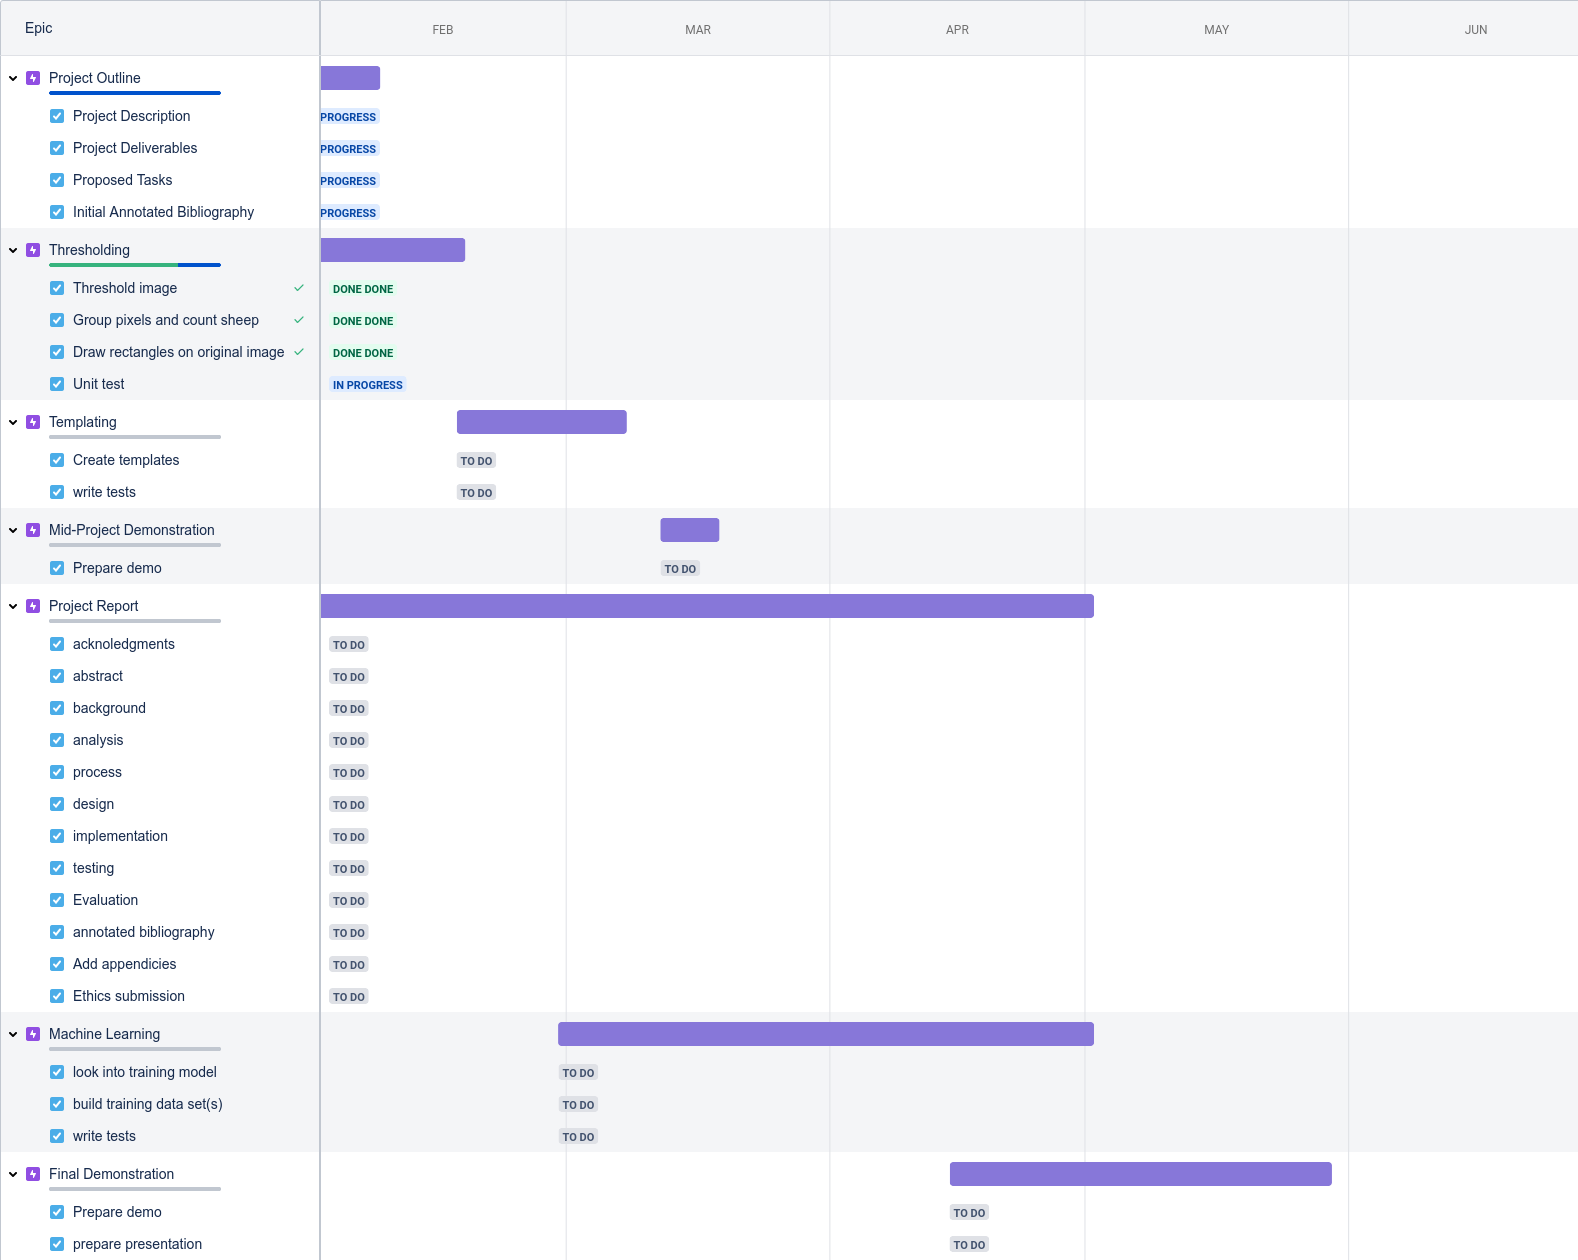
\includegraphics[width=0.9\textwidth]{where_smysheep_2020-02-07_0958am.png}
\end{figure}


%==============================================================================
\section{Project Deliverables}
%==============================================================================
\begin{itemize}
    \item Project Outline, this document
    \item Project Report
    \item Python OpenCV script with thresholding attempt, for white sheep.
    \item Python OpenCv script with templating attempt.
    \item Tests for the thresholding and templating attempt
    \item Mid project Demo
    \item Tensorflow model with scripts to apply it to image.
    \item Tests for the final code
    \item Final Demo
\end{itemize}


%
% Start to comment out / remove the following lines. They are only provided for instruction for this example template.  You don't need the following section title, because it will be added as part of the bibliography section.
%
%==============================================================================
%\section*{Your Bibliography - REMOVE this title and text for final version}
%==============================================================================
%
%You need to include an annotated bibliography. This should list all relevant web pages, books, journals etc. that you have consulted in researching your project. Each reference should include an annotation.

%The purpose of the section is to understand what sources you are looking at.  A correctly formatted list of items and annotations is sufficient. You might go further and make use of bibliographic tools, e.g. BibTeX in a LaTeX document, could be used to provide citations, for example \cite{NumericalRecipes} \cite{MarksPaper} \cite[99-101]{FailBlog} \cite{kittenpic_ref}.  The bibliographic tools are not a requirement, but you are welcome to use them.

%You can remove the above {\em Your Bibliography} section heading because it will be added in by the renewcommand which is part of the bibliography. The correct annotated bibliography information is provided below.
%
% End of comment out / remove the lines. They are only provided for instruction for this example template.
%


\nocite{*} % include everything from the bibliography, irrespective of whether it has been referenced.

% the following line is included so that the bibliography is also shown in the table of contents. There is the possibility that this is added to the previous page for the bibliography. To address this, a newline is added so that it appears on the first page for the bibliography.
\newpage
\addcontentsline{toc}{section}{Initial Annotated Bibliography}

%
% example of including an annotated bibliography. The current style is an author date one. If you want to change, comment out the line and uncomment the subsequent line. You should also modify the packages included at the top (see the notes earlier in the file) and then trash your aux files and re-run.
%\bibliographystyle{authordate2annot}
\bibliographystyle{IEEEannotU}
\renewcommand{\refname}{Annotated Bibliography}  % if you put text into the final {} on this line, you will get an extra title, e.g. References. This isn't necessary for the outline project specification.
\bibliography{mmp} % References file

\end{document}
